% Define document class
\documentclass[twocolumn]{aastex631}
\usepackage{showyourwork}
\usepackage[version=4]{mhchem}
\usepackage{listings}


\newcommand{\teff}{$T_{\rm eff}$}
\definecolor{tedcommentcolor}{HTML}{e17701}
\newcommand{\TJ}[1]{\textcolor{tedcommentcolor}{#1}}
\newcommand{\vspec}[1]{\texttt{VSPEC}#1}
% \def\vspec#{\texttt{VSPEC}}

\shorttitle{\vspec{}}
\shortauthors{Johnson et al.}

% Begin!
\begin{document}

% Title
% \title{The \vspec{} code: Spectroscopic phase curves of 3D exoplanet models in the presence of stellar variability}
\title{\vspec{} and Friends: A suite of utilities to model spectroscopic phase curves of 3D exoplanet atmospheres in the presence of stellar variability.}

\author{Ted Johnson}
\affiliation{NASA Goddard Space Flight Center \\
8800 Greenbelt Rd \\
Greenbelt, MD 20771, USA}
\affiliation{Nevada Center for Astrophysics, University of Nevada, Las Vegas, 4505 South Maryland Parkway, Las Vegas, NV 89154, USA}
\affiliation{Department of Physics and Astronomy, University of Nevada, Las Vegas, 4505 South Maryland Parkway, Las Vegas, NV 89154, USA}
% Also CRESST, SURA, SEEC!

\author{Cameron Kelahan}
\affiliation{NASA Goddard Space Flight Center \\
8800 Greenbelt Rd \\
Greenbelt, MD 20771, USA}

\author{Avi M. Mandell}
\affiliation{NASA Goddard Space Flight Center \\
8800 Greenbelt Rd \\
Greenbelt, MD 20771, USA}

\author{Tom Barclay}
\affiliation{NASA Goddard Space Flight Center \\
8800 Greenbelt Rd \\
Greenbelt, MD 20771, USA}

\author{Veselin B. Kostov}
\affiliation{NASA Goddard Space Flight Center \\
8800 Greenbelt Rd \\
Greenbelt, MD 20771, USA}

\author{Geronimo L. Villanueva}
\affiliation{NASA Goddard Space Flight Center \\
8800 Greenbelt Rd \\
Greenbelt, MD 20771, USA}

% Abstract with filler text
\begin{abstract}
    We present the Variable Star Phase Curve (\href{https://github.com/VSPEC-collab/VSPEC} \vspec{}) code,
    a python package to simulate combined-light spectroscopic observations of exoplanets in the presence of stellar variability and inhomogeneity.
    \vspec{} uses the Planetary Spectrum Generator's Global Emission Spectra (PSG GlobES) application along with a custom-built
    stellar model based on an existing grid of stellar photosphere models to produce spectroscopic light curves of the planet-host system.
    \vspec{} can be a useful tool for modeling observations of exoplanets in transiting geometries (primary transit, secondary eclipse) as well as orbital phase curve measurements,
    and is built in a modular and flexible configuration for easy adaptability to new stellar and planetary model inputs. We additionally present
    a set of codes developed alongside \vspec{}, including the stellar surface model \texttt{vspec-vsm}, the stellar spectral grid interpolation code
    Gridpolator, and a Python interface for PSG \texttt{pypsg}.
\end{abstract}

\keywords{Exoplanet, M dwarf}

% Main body with filler text
\section{Introduction}
\label{sec:intro}

In the era of high-sensitivity exoplanet characterization missions such as the James Webb Space Telescope (JWST)
and the Atmospheric Remote-sensing Infrared Exoplanet Large-survey (ARIEL), spectral analysis of exoplanet atmospheres
is increasingly sensitive to contamination due to stellar inhomogeneities (e.g. spots, granulation) and stochastic stellar variability (e.g. flares).

Recent analysis of the JWST/NIRSpec transit of GJ 486b by \citet{moran2023} exposed a degeneracy between
atmospheric absorption by water and water-rich spots on the stellar surface. This ``transit light source effect''
\citep[TLS,][see also \citet{apai2018,barclay2021,garcia2022,barclay2023}]{rackham2018}
occurs when the occulted region of the stellar surface is not representative of the disk-integrated spectrum.

Similarly, the Mid-IR Exoplanet CLimate Explorer \citep[MIRECLE,][]{mandell2022} mission concept
will employ the Planetary Infrared Excess \citep[PIE][]{stevenson2020} technique to extract the planetary
contribution from combined-light observations. Uncertainties on the stellar spectrum will dominate the analysis if it is not removed appropriately.

To adequately prepare for future observations and future missions it will be necessary to demonstrate a method to mitigate these effects.
This task requires a flexible tool that combines models of exoplanet atmospheres and stellar variability in a robust way.

In this paper we present \vspec{}: Variable Star PhasE Curve\footnote{\url{https://github.com/VSPEC-collab/VSPEC}},
an open-source Python 3 package to simulate observations of exoplanet systems with variable host stars.
\vspec{} itself is merely an interface that pulls together a variable star surface model \texttt{vspec-vsm}\footnote{\url{https://github.com/VSPEC-collab/vspec-vsm}},
a stellar spectra grid interpolation code Gridpolator\footnote{\url{https://github.com/VSPEC-collab/GridPolator}}, and a Python interface for
the Planetary Spectrum Generator \citep[PSG,][]{villanueva2018}, \texttt{pypsg}. All of these codes together allow \vspec{} to account for
3D planetary atmospheres, time-resolved effects of both planet and star, many geometries including transit and eclipse, and realistic noise modeling.

\TJ{Change this later-->}
In this paper we will describe the science behind \vspec{} and demonstrate examples of its use.
Section \ref{sec:star} describes the stellar model and the available sources of variability.
Section \ref{sec:pl_model} discusses modeling the planetary atmosphere, including PSG/GlobES and the
built-in GCM. In Section \ref{sec:examples} we provide examples of \vspec{} use cases and demonstrate
its value to the exoplanet community. Finally, in Section \ref{sec:conclusion} we will discuss the future of the code and issues it might have.

\section{Using \vspec{}}
\label{sec:vspec}

The flow of \vspec{}'s code is broken into three parts: i) read in the configuration, ii) compute planetary spectra, and iii) compute stellar spectra.
\subsection{Configuring \vspec{}}
\label{subsec:config}

\vspec{} configurations are designed to minimize human errors by providing two equivalent formats. The first, a file written in YAML, is optimized for
human readability. For example, the \texttt{system} section, which describes the relationship between the observed planetary system and the observer, could
be written:
\begin{lstlisting}[label={ls:yaml}]
system:
    distance: 12.4 pc
    inclination: 89.7 deg
    phase_of_pariasteron: 0 deg
\end{lstlisting}
Note that the units of each of these parameters is included in a human-readable way. Internally, \vspec{} casts each of these parameters to an Astropy
\texttt{Quantity} instance, so that the user can input any desired value and unit combination so long as the physical type is correct -- i.e. it would be
equivalent to write \texttt{3.83e17 m} as the value for the \texttt{distance} parameter.

The second input method available is to directly initialize the Python object that \vspec{} uses internally to store its model parameters.
The top-level object, \texttt{InternalParameters}, is structured to mirror the YAML input file, with one argument per YAML section. The
parameters in Listing \ref{ls:yaml} would be written:
\begin{lstlisting}[language=Python]
from astropy import units as u
from VSPEC.params import *
params = InternalParameters(
    ... # Other arguments
    system=SystemParameters(
        distance=12.4*u.pc,
        inclination=89.7*u.deg,
        phase_of_pariasteron=0*u.deg
    )
)
\end{lstlisting}
This is convenient for producing configurations programically, for example for producing a grid of model phase curves.

However the user decides to provide model parameters, they are read into the main \vspec{} object: the \texttt{ObservationModel}.
This is the class that runs the model and handles files. Upon initialization a local working directory
(by convention \texttt{.vspec}) is created to store simulation outputs and intermediate files.

\subsection{Planetary Phase Curve}
\label{subsec:phase-curve}
\vspec{} generates a phase curve though a series of API calls to the Planetary Spectrum Generator \citep[PSG][]{villanueva2018}, using
\texttt{pypsg} (see Section \ref{sec:pypsg}) to interface with the API. Initially, configurations are sent that give PSG information about
the system that does not change with time -- that includes the 3D Global Circulation Model (GCM) and instrument parameters. \vspec{} then enters
the main loop, iterating through each observation epoch and making a pair of API calls: one to get a combined light spectrum and one to get the thermal flux only.
Results from PSG in each epoch are stored locally in the \texttt{.fits} format. 

\subsubsection{Phase Sampling}
Making API calls to PSG can be computationally expensive, especially when trying to resolve small structures in the climate model. In order to reduce unnecessary
calls to PSG the temporal sampling of the planetary spectrum in independent of the stellar model/output sampling. When computing the planetary flux in the output files
the raw PSG output is interpolated and averaged over the integration using the trapazoid rule. By default one spectrum is computed at each interface separating integrations.

\subsection{Stellar Lightcurve}

The last step is to replace the stellar spectra used by PSG with \vspec{}'s stellar model. In this step \vspec{} acts as a bridge between
the stellar surface model \texttt{vspec-vsm} (which models spatial changes to the star with time, see Section \ref{sec:star}) and a grid of
pre-computed stellar spectra (see Section \ref{sec:gridpolator}). The star is initialized and allowed to evolve for a user-specified amount of time
in order for spots and faculae to approach growth-decay equilibrium (this is also called the ``burn in'' phase). The star is then evolved at the output cadence,
at each epoch generating a set of key-value pairs that describe the surface temperature and coverage fractions of the portion of the stellar disk visible to the observer.
These \teff\ s and coverage fractions are fed into GridPolator to produce composite stellar spectra.

\subsubsection{Reflected light}
\vspec{} also produces a composite spectrum of the
portion of the star visible to the planet to accurately incorporate the variable star into the reflected light spectrum. To compute the total reflected light
in the output files \vspec{} first divides the reflected light flux from PSG by the PSG stellar model to obtain the apparent albedo. This albedo is then multiplied
by the composite spectrum (facing the planet) to obtain total reflected light flux.

\subsubsection{Noise}
Alongside the planetary radiance files PSG returns a file giving the noise profile for each epoch broken down by source. We assume that the total noise is the
quadrature sum of its constituent parts and that the \texttt{source} column (i.e. photon noise) is the only one effected by replacing one stellar spectrum with the other.
This means the photon noise can be calculated:
\begin{equation}
    N_{\rm photon} = N_{\rm photon,~PSG} \sqrt{\frac{F_{*,\rm ~VSPEC}}{F_{*,\rm ~PSG}}}
\end{equation}
where $F_*$ is the stellar flux. The total noise associated with the integration is then
\begin{equation}
    N_{\rm tot} = \sqrt{
        N_{\rm photon}^2 + N_{\rm detector}^2 + N_{\rm telescope}^2 + N_{\rm background}
    }
\end{equation}

\subsubsection{Transit and Eclipse}
Users must be careful when using \vspec{} to simulate transit and eclipse measurements because of the vast timescale differences between those events
and the typical phase variations of the planet -- a sparsely sampled phase curve that happens to include one epoch of transit will not describe that lightcurve accurately
because the interpolator knows no better than to assume a linear interpolation scheme. It is recommended that users use a high cadence for observations of transits
and eclipses so that each event will be sampled by more than one point.

In the case of a transiting geometry \vspec{} computes the spectrum of the occulted portion of the star in order to properly simulate the
transit light source effect \citep[TLS][]{rackham2018}. This spectrum is the flux blocked by the planet in the case that it is a bare rock (i.e. a flat
transmission spectrum). The effect of atmospheric transmission is added by comparing the PSG-computed effective radius to a purely geometric
calculation of a bare-rock transit depth. That is
\begin{equation}
    F_{\lambda} = F_{{\rm rock}, \lambda}\, F_{{\rm PSG,} \lambda} \,\left (\frac{R_*}{R_p} \right )^2
\end{equation}
where $F_\lambda$ is the flux of the variable star surface occulted by the planet with the atmosphere considered. $F_{{\rm rock}, \lambda}$ is the
flux of the surface occulted by a bare-rock with the planet's radius, $F_{{\rm PSG,} \lambda}$ is the flux computed by PSG to be lost
due to occultation and transmission, and $R_*$ and $R_p$ are the stellar and planetary radii, respectively.

In the case of a total eclipse of the planet the thermal and reflected spectra are set to zero flux. However, in the case of a partial eclipse,
\vspec{} computes the fraction of the planet that is visible to the observer and reduces both thermal and reflected spectra accordingly. In this case
\vspec{} treats the planet homogeneously, however future work could utilize PSG/GlobES's ability to return a hypercube of spatially resolved
spectra in order to construct planetary spectra only from regions of the planet that are not eclipsed.

\subsection{Analysis Tools}
The final outputs of \vspec{} should be easily read using Astropy's \texttt{QTable} object, but we have also included a class \texttt{PhaseAnalyzer} to automatically
parse all output files and conveniently access 1D spectra or lightcurves. \TJ{Is it worth talking about this?}

\section{Interfacing with the Planetary Spectrum Generator via \texttt{pypsg}}
\label{sec:pypsg}

PSG\footnote{\url{https://psg.gsfc.nasa.gov/}} \citep{villanueva2018} is a powerful radiative transfer tool that is ubiquitous in the exoplanet and solar system atmosphere fields.
Either though its web graphical interface, its public API, or the local version available through Docker, PSG allows users to simulate observations of planets, comets, and
moons with a variety of geometries and realistic noise models \TJ{probably someone like Geronimo should write this part}.

During development of \vspec{} it became clear that a Python interface for the PSG API system would be generally useful to planetary scientists and astronomers, and
so \vspec{}'s own interface was spun off into a stand-alone library: \texttt{pypsg}.

\texttt{pypsg} draws inspiration from object-relational mapping in frameworks such as Django to encode a PSG configuration file as a native Python object.
Fields of a \texttt{pypsg} data model represent one or more lines of a configuration file, and the two representations are interchangable without loss of information.

Upon creation of this configuration as a \texttt{PyConfig} object, a user can create an \texttt{APICall} instance which handles sending a request to PSG via Python's
\texttt{requests} package. This dedicated caller is important in that it reads a user's API key from a known location on disk, removing the possibility that the key
could be committed to a public repository.

\subsection{GlobES}
\label{subsec:globes}

A powerful feature of \texttt{pypsg} is that it provides a universal interface for 3D atmosphere models and PSG's Global Emission Spectra (GlobES) application.
GlobES expects 3D data to be presented in a binary data format, and converting a model to this format is non-trivial. \texttt{pypsg}'s \texttt{PyGCM} class provides
a native Python representation of GlobES input, and includes built-in methods for converting popular climate models (e.g. ExoCAM, WACCM \TJ{full names and ref?}) to
the correct format.

\section{Stellar Model}
\label{sec:star}

The \vspec{} star model is designed modularly to allow
for both simple and complex behaviors. Currently, it
is represented by a rectangular grid of points on the stellar surface,
each assigned an effective temperature. At any given time, the model computes
the surface coverage fractions of each temperature visible to the observer, accounting for the
spherical geometry, limb darkening, and any occultation by a transiting planet.

The attributes of the \texttt{Star} class describe the bulk properties of the star, including radius,
period, and the effective temperature of quiet photosphere. Herein we refer to this temperature as the
photosphere temperature to differentiate it from the temperature of spots, faculae, or other sources of variability.

\begin{figure}
    \centering
        \includegraphics[width=0.5\textwidth]{figures/surface_map_and_lc.pdf}
    \script{surface_map_and_lc.py}
    \caption{{\bf Top}: The surface map of a star with spots and faculae during a transit.
    The large circles are spots. Faculae display their 3D structure, as the hot wall is more prevalent near the limbs.
    {\bf Bottom}: An example lightcurve of a spotted star.}
    \label{fig:surface_map}
\end{figure}

\subsection{Stellar Spectra \label{subsec:spectra}}
Once the surface coverage is calculated, a composite spectrum is computed from a grid of PHOENIX stellar spectra
\citep{husser2013}.
As of \texttt{VSPEC 0.1} \TJ{fix!}, we have spectra between 2300 K and 3900 K, with steps of
100 K. Each spectrum has $\log{g} = 5$ and solar metalicity.
The raw spectra span from 0.1 to 20 \micron~ with $5 \times 10^{-6}$ \micron~ steps, however binned
versions are pre-computed for faster runtimes.

\subsection{Spots \label{subsec:spots}}
Our star spot model is nearly entirely based on observations of the sun. Sun spots can be resolved and are well-studied,
whereas spots on other stars (e.g., M dwarfs) can only be observed indirectly. We therefore designed our spot model to mimic
sun spots but with parameterized values for spot temperature and lifetime that can be matched to observations of other stellar types and ages.


On the Sun, spots have two regions: the dark, central umbra and the lighter, surrounding penumbra. A detailed review of sunspot behavior,
including sizes and lifetimes, is \citet{solanki2003}, however the specific solar values are not relevant to this description. However,
the spot area as a function of time is
\begin{equation}
    A(t) = \left\{
    \begin{array}{lr}
        A_0 e^{(t-t_0)/\tau}, & \text{if } t \leq t_0 \\
        A_0 - W(t-t_0), & \text{if } t > t_0
    \end{array}
    \right\}
\end{equation}
where $A_0$ is the maximum area reached, $t_0$ is the time of the maximum, $\tau$ is the exponential growth rate, and $W$ is the linear decay rate.

\vspec{} also takes in parameters describing the population of spots, such as the mean of the (lognormal) peak area distribution
\citep{bogdan1988}, the equilibrium surface coverage, and the distribution style.

\subsection{Faculae \label{subsec:faculae}}
Faculae are magnetically-generated regions of the solar surface that usually appear as bright points near the limb; we employ the ``hot wall''
model \citep{spruit1976} where faculae are described as three-dimensional pores in the stellar surface with a hot, bright wall, and a
cool, dark floor, as shown in Figure \ref{fig:fac_struct}.

Their three-dimensional structure causes faculae to behave differently depending on their angle from disk-center. Close to the limb,
the hot wall is visible to the observer, and faculae appear as bright points. Near the center, however, the cool floor is exposed and
faculae appear dark. To consider this effect in the faculae lightcurve, we compute the fraction of the facula's normalized area -- the
area on the disk it would occupy as a flat spot -- that is occupied by each the hot wall and cool floor. This is done via numerical integral
along the radius of the spot.

\begin{equation}
    f_{wall} = \frac{\int _{-R}^{R} Z_{\rm eff} dr}{\int _{-R}^{R} Z_{\rm eff} dr + \int _{-R}^{R} R_{\rm eff} dr}
\end{equation}
where $Z_{\rm eff}$ is the apparent height of the wall
\begin{equation}
    Z_{\rm eff} = \left\{
    \begin{array}{lr}
        Z_w \sin{\alpha}, & \text{if } \alpha \leq \alpha_{\rm crit} \\
        2\sqrt{R^2 - r^2}\cos{\alpha}, & \text{if } \alpha > \alpha_{\rm crit}
    \end{array}
    \right\}
\end{equation}
and $R_{\rm eff}$ is the apparent width of the floor
\begin{equation}
    R_{\rm eff} = \left\{
    \begin{array}{lr}
        2\sqrt{R^2 - r^2} - Z_w\sin{\alpha}, & \text{if } \alpha \leq \alpha_{\rm crit} \\
        0, & \text{if } \alpha > \alpha_{\rm crit}
    \end{array}
    \right\}
\end{equation}
for facula radius $R$, depth $Z_w$, and angle from disk-center $\alpha$. $r$ in this numerical scheme
is defined as the distance from the center of the facula along the radial line connecting the facula center to the
disk center. $\alpha_{\rm crit}$ is the value of alpha at which the floor is no longer visible and is defined to be $\arctan{\frac{2\sqrt{R^2-r^2}}{Z_w}}$.

According to \citet{1997ApJ...484..479T}, faculae temperatures (of both the floor and wall) are dependent on the facula radius,
while depth appears to be constant. They also find that the smallest faculae have no visible floor, and that even at disk center they
appear as bright points. We parameterize the floor temperature to be
\begin{equation}
    \Delta T_{\rm eff, floor} = \left\{
    \begin{array}{lr}
    \text{Not visible}, & \text{if } r<r_{\rm min} \\
    m_{\rm floor}(r-r_{\rm min}) + \Delta T_{\rm eff, floor, 0}, & \text{if } r \ge r_{\rm min}
    \end{array}
    \right\}
\end{equation}

Where $r$ is the radius of the facula, $r_{\rm min}$ is the minimum radius where the floor is visible, $\Delta  T_{\rm eff, floor, 0}$ is
the difference between the floor and photosphere \teff at $r_{\rm min}$, and $m_{\rm floor}$ is the slope of the relationship with
units of [temperature] [length]$^{-1}$.

Similarly, the wall temperature is parameterized

\begin{equation}
    \Delta T_{\rm eff,wall} = m_{\rm wall}r + \Delta T_{\rm eff,wall,0}
\end{equation}

Where $\Delta T_{\rm eff,wall,0}$ is the temperature of a zero-radius facula and and $m_{\rm wall}$ is the slope of the radius-temperature
relationship with units of [temperature] [length]$^{-1}$.
These relationships can be defined by the user, for example setting $m=0$ for constant temperatures.

Facula lifetimes are defined as the time it takes to decay by $e^{-2}$. Because faculae grow and decay exponentially
at the same rate, each facula spends 1 lifetime with a radius greater than $e^{-1}$ of it's maximum. Each facula is born
and dies at $e^{-2}$ of its maximum, effectively existing in the code for two lifetimes.

\citet{hovis-afflerbach2022} suggest a typical facula lifetime to be on the order of 6 hours,
with a distribution that resembles a Poisson function. However, we choose a lognormal distribution
for both lifetime and maximum radius because it does not allow for these values to be 0. We choose to
correlate lifetime and radius so that they are determined by the normally distributed random variable $\mu$;
for each new facula, $\mu$ is randomly drawn and determines both the faclue lifetime and maximum radius.

\begin{figure}
    \centering
    \gridline{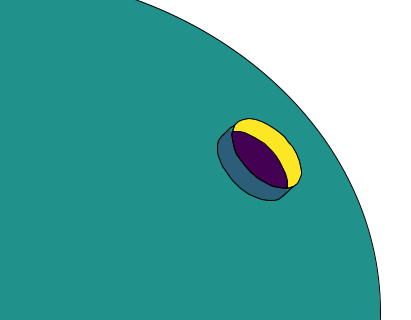
\includegraphics[width=0.5\textwidth]{figures/facula_model.png}}
    \gridline{\includegraphics[width=0.5\textwidth]{figures/facula_depth.pdf}}
    \script{facula_depth.py}
    \caption{
        ``Hot Wall'' model of faculae. Faculae structure causes their contrast to be dependent on their distance
        from the center of the disk. {\bf Top}: Depiction of a facula on the limb of a star. The hot wall is exposed
        to the observer causing the pore to appear bright. At disk center, the cool floor is most visible. {\bf Bottom}:
        The effects of depression depth and viewing angle on facula brightness. The 3D structure of faculae is most apparent
        when radius $\sim$ depth. A toy flux model was used to demonstrate the shape of these curves, but their magnitudes
        in practice depend on stellar spectral models.
        }
    \label{fig:fac_struct}
\end{figure}

\subsection{Flares \label{subsec:flares}}
Flares are an important source of stellar variability on short timescales. We use the {\sc xoflares}
package \citep{barclay2020} to generate realistic lightcurve shapes and assume a blackbody spectrum.
{\sc xoflares} uses a flare profile function empirically derived by \citet{davenport2016} to
describe a flare lightcurve. Temperature, $E$, FWHM, and the peak time together completely describe a flare's multiwavelength lightcurve.

Before simulating an observation, \vspec{} pre-computes a population of flares based on the frequency-energy relationship from \citet{gao2022}:
\begin{equation} \label{eq:flare_freq}
    \log{(f{\rm [day]})} = \beta + \alpha~\log{(E/{\rm [erg]})}
\end{equation}

Where $f$ is the frequency of flares with energies $\ge E$.
We compute the number of expected flares over a time duration and determine the number to create $N$ by a random Poisson draw.
We then generate $N$ flares with energies determined by the quantile function:
\begin{equation}
    E = E_{\text{min}} (1-X)^{1/\alpha}
\end{equation}

where $E_{\text{min}}$ is the minimum considered flare energy and $X$ is a random number on the interval $[0,1)$.
We set the default values $\alpha=-0.829$, $\beta=26.87$ from \citet{gao2022}. Figure \ref{fig:flare_freq}
shows our simulation results compared to their powerlaw.

\begin{figure}
    \centering
    \includegraphics[width=0.5\textwidth]{figures/flare_freq.pdf}
    \caption{
        {\bf Top}: Generated flare frequencies compared to those expected from \citet{gao2022}, generated using a 10,000 day simulation.
        The $y$-axis shows the frequency of flares with energies {\em greater than or equal to} the value of the $x$-axis. Error bars
        based on the square root of the number of observed flares as this is a Poisson process.
        {\bf Bottom}: Lightcurve of a star flaring with the same powerlaw slope as the top panel, but the intercept ($\beta$) has been increased by 0.3
        for visual effect. The mean flare temperature is $9000$ K and the mean FWHM is $3$ hours.
        }
    \script{flare_freq.py}
    \label{fig:flare_freq}
\end{figure}

\subsection{Granulation}
Granulation is a source of stellar variability that arises from convection near the surface of the star.
The result is a stellar surface that is not constant in temperature and that changes on very short timescales.
Hydrodynamic simulations of stellar atmospheres \citep[e.g.][]{magic2014} describe hot granules of rising gas surrounded by cooler,
sinking regions with a \teff a few percent lower than the nominal value.

We model granulation as a global process, and its effects are computed after the effects of spots and faculae.
Of the remaining ``quiet'' photosphere (i.e. the regions not covered in spots of faculae), a fraction is computed to be part of the cool
inter-granule surface. The surface coverage of the cool region at any given time is computed by a Gaussian process (GP) using
the {\sc tinygp} package \citep{foreman-mackey2024} following the methodology of \citet{gordon2020}.
The GP uses a custom kernel function based on a power spectrum \citep{anderson1990,kallinger2014} to produce random changes in the coverage.

\begin{figure}
    \centering
    \includegraphics[width=0.5\textwidth]{figures/granulation_lightcurve.pdf}
    \caption{
        Effect of granulation on the lightcurve of a star. This simulation assumes a mean
        10\% coverage by inter-granule region whose temperature is 300 K lower than the surrounding photosphere.
        It also assumes that the coverage value varies with a magnitude of 1\% on a timescale of 6 hours.
        }
    \script{granule_lc.py}
    \label{fig:gran_lc}
a\end{figure}

\section{Planet Model \label{sec:pl_model}}
Our model uses the Planetary Spectrum Generator\footnote{\href{https://psg.gsfc.nasa.gov/}{https://psg.gsfc.nasa.gov/}}
\citep[PSG,][]{villanueva2018} to calculate the planetary spectrum. We upload a 3D Global Circulation Model (GCM) to PSG's
Global Emission Spectra (GlobES) application to retrieve thermal and reflected spectra for various points in the planet's phase curve. \TJ{cite Vincent's paper}

\subsection{Interfacing through {\sc pypsg}}
\ref{subsec:pypsg}
\vspec{} interfaces with PSG using the {\sc pypsg} package \TJ{link}, which is essentially a Python wrapper for the PSG API system.

\TJ{Write much more}

\subsection{3D Planet models}
\vspec{} allows the user to upload any desired GCM. However, for questions that focus on detectability,
the specific physics of the GCM are less important than properties like day/night temperature, surface pressure, or
the major absorbers in the atmosphere. To simplify these studies, \vspec{} has a built-in GCM that takes in just a
few parameters and produces a simple-yet-robust exoplanet climate. Simplicity allows the user to know everything about
the model and reduce surprises, but its basis in thermodynamics and robust energy balance make this model fit for publication-level science \TJ{is this really true? probably not}.

The \vspec{} GCM centers around a 2D temperature map of the planet's surface. Based on \citet{cowan2011}, this map
is constructed completely given the incident flux from the star (parameterized by the host \teff and radius
and the planet's semimajor axis and Bond albedo) and the unitless thermal redistribution efficiency $\epsilon$.
This efficiency is 0 for a planet that reradiates instantly and $\gg 1$ for an atmosphere that efficiently redistributes heat to its night side.
Figure \ref{fig:thermal_inertia} shows a temperature map example for an Earth-like planet with $\epsilon = 2\pi$.
These temperature maps are validated by the energy balance of the planet; \vspec{} computes the incident and emergent
flux across the planet and asserts that they agree.

\begin{figure}
    \centering
    \includegraphics[width=0.5\textwidth]{figures/cowan_gcm.pdf}
    \caption{
        Example of a surface temperature map created by \vspec{}. The solar flux at Earth,
        a Bond albedo of 0.3, and $\epsilon = 2\pi$ were used in this case.
        Notice that the hottest point is offset from the sub-stellar point due to thermal inertia.
    }
    \script{cowan_gcm.py}
    \label{fig:thermal_inertia}
\end{figure}

Now that we have the surface temperature at each GCM coordinate we can build the atmosphere on top of it.
We choose a surface pressure for our model and generate a pressure profile as a function of layer. It is
important to note that the choice of the pressure profile -- provided it is scaled to the surface pressure and sampled in a reasonable manner -- is
arbitrary and will not affect the spectrum of the planet. This is because PSG calculates the altitude and thickness of each layer based on the
pressure and surface gravity; the pressure profile is essentially a proxy for the sampling of atmosphere layers as a function of altitude.

Next we create an adiabatic temperature profile at each GCM coordinate. An adiabat assumes that
\begin{equation}
    T^\gamma P^{1 - \gamma} = \text{const.}
\end{equation}
where $\gamma$ is the adiabatic index. Therefore the temperature profile can be computed
\begin{equation}
    T = T_{\rm surf} \left(\frac{P}{P_{\rm surf}} \right)^{1 - \frac{1}{\gamma} }
\end{equation}

Finally, we populate our atmosphere with molecules. The user specifies the species and abundance and atmosphere is filled accordingly with a constant molecular suite.

The caveats of this approach lie in the simplified physics of the atmosphere structure. The heat-redistribution model does not
capture the effects of latitudinal mixing; an adiabatic temperature profile will never exhibit the temperature inversion
that we know form in complex atmospheres like Earth's. Similarly, setting a constant abundance does not allow for water vapor to
vary with temperature as it does on Earth. We must also be careful not to add so much of an absorbing species that the energy balance of
the atmosphere would change; instead we treat them as trace species in an otherwise transparent atmosphere. Our simplified approach
allows us to easily examine a large parameter space of atmospheres whose behaviors are easy to predict.

\section{Examples \label{sec:examples}}

\subsection{Transit of a spotted star}

In this section we will simulate the transit of a bare rock across a spotted star to demonstrate how an inhomogeneous
stellar surface can lead to a false atmospheric signal -- a phenomenon known as the ``transit light source effect'' \citep{rackham2018}.
During transit, the planetary atmosphere is illuminated by the portion of the star directly behind the planet. The depth of the transit
should be measured with respect for the spectrum of this region of the stellar surface. However, the disk-integrated stellar spectrum is often used instead.
In the case that the stellar surface is not homogeneous, the transit signal is contaminated by the star.
\citet{moran2023} first observed this effect using JWST from super-Earth GJ 486b.

Whenever possible, we draw parameter values from \citet{moran2023} and the NExScI Archive\footnote{\url{https://exoplanetarchive.ipac.caltech.edu/overview/GJ1214b}}.
We use the JWST NIRSpec/G395H instrument setup but set $R=200$ to account for the resolution of the reduction.
Additionally we observe for 3.53 hours with an 8 minute cadence. Mid-transit is reached exactly halfway through the observation.

We will do three \vspec{} simulations:
\begin{enumerate}
    \item Bare rock, no spots.
    \item 1 bar \ce{H2O} atmosphere, no spots.
    \item Bare rock, 2.5\% coverage by 2700 K spots
\end{enumerate}

We expect in case 1 to observe a flat spectrum, and in case 2 to observe additional
absorption from the \ce{H2O} atmosphere. Note also that we disabled \ce{H2O}-\ce{H2O} collision-induced absorption (CIA) for
these simulations because the effect was not considered in the original analysis of GJ 486b.

\begin{figure}
    \centering
    \includegraphics[width=0.5\textwidth]{figures/moran23.pdf}
    \caption{
        The results from our spotted transit experiment. We find that the addition of
        spots to a star's surface can give an otherwise flat transit spectrum features that appear to be molecular bands.
        This is in agreement with the results of \citet{moran2023}.
        }
    \script{moran23.py}
    \label{fig:moran_transit}
\end{figure}

We find that, as expected, the addition of spots changes the transit depth in a way that depends on wavelength -- mimicking
light lost to absorbers in a planetary atmosphere. Figure \ref{fig:moran_transit} shows us that, in this case, we observe false absorption;
this is due to an increase in the spotted fraction of the surface relative to the quiet photosphere. However, if a spot was blocked by
the planet we might see similar features inverted to mimic emission.

\subsection{Phase Curve}
Analysis of JWST MIRI-LRS phase curves of GJ 1214b by \citet{kempton2023} did not consider stellar
contamination because of the slow rotation rate of the host star \citep[approximately 1/80$^{\text{th}}$ the orbital frequency,][]{cloutier2021}.
In this example we use \vspec{} to demonstrate that this is a reasonable assumption.

We initialize \vspec{} to run a 41.0 hour observation with a cadence of 15 minutes. We use stellar and planetary parameters
from the NExScI Exoplanet Archive\footnote{\url{https://exoplanetarchive.ipac.caltech.edu/overview/GJ1214b}}.
The GCM used has a thermal inertia of $\epsilon = 6$ and a 1 bar \ce{CO2} atmosphere.

We initialized two stellar models: one with nothing more than a 3250 K surface, and another with 20\% coverage by 2700 K spots.

After running the \vspec{} simulations, we bin into 0.5 $\mu m$ wavelength channels and normalize each channel to the two eclipses.
We assume the star behaves linearly between eclipse measurements and attribute any deviation to the planet.

\begin{figure}
    \centering
    \includegraphics[width=0.5\textwidth]{figures/kempton23.pdf}
    \caption{
        MIRI phase curves for GJ 1214b binned by wavelength. Compare to \citet{kempton2023} Extended Data Figure 1.
        While the addition of stellar variability does have a visible effect on the lightcurve, it is much smaller than the thermal emission by the exoplanet.
        }
    \script{kempton23.py}
    \label{fig:gj1214b}
\end{figure}

We show in Figure \ref{fig:gj1214b} that the stellar properties assumed in this example do not generate enough contamination to
significantly change the observed phase curve of GJ 1214b. At it's worst (i.e. near transit) the observed spectrum varies by 50 ppm due to stellar
contamination -- compared to the 700 ppm relative flux of the planet at $8.5 {\mu m}$. Similar studies could be done to assess the potential for
stellar contamination in other exoplanetary systems in order to judge fitness as a target.

\subsection{MIRECLE Phase Curve}
In this example we will look at the best-case target for the Mid-IR Exoplanet CLimate Explorer \citep[MIRECLE,][]{mandell2022}
mission concept: Proxima Centauri b with no stellar variability. We will instead examine the expected noise produced by this observation
and assess the detectability of the planet in a single orbit. \vspec{} uses the noise models built into PSG, allowing native support for
noise due to the instrument, source, and astrophysical background.

We use \vspec{}'s built-in MIRECLE instrument template, which includes a 2 m aperture and observes from 1-18 $\mu m$ with $R=50$.
We draw stellar and bulk planetary parameters from the NExScI Exoplanet Archive\footnote{\url{https://exoplanetarchive.ipac.caltech.edu/overview/proxima\%20cen}}
and assume $i=85^\circ$ and Earth density. The GCM we use has a Bond albedo of 0.3, $\epsilon=1.5$, $P_{\rm surf} = 1 \text{bar}$ and a 100 ppm \ce{CO2} atmosphere with a \ce{N2} background.
We ran the simulation for one orbit with an 24 hour cadence. Because this is a best-case scenario, we assumed perfect knowledge of the stellar spectrum.
We are left with the planetary spectrum and photon noise from the star.

\begin{figure}
    \centering
    \includegraphics[width=0.5\textwidth]{figures/mirecle.pdf}
    \caption{
        Simulated spectra of Proxima Centauri b observed by MIRECLE. Noise and error bars based on 24 hour integrations with a 2 m aperture MIRECLE
        space telescope.
        }
    \script{mirecle.py}
    \label{fig:mirecle}
\end{figure}

\section{Conclusion \label{sec:conclusion}}
\TJ{Talk about what we can do next.}

\bibliography{syw,VSPEC}

\end{document}
